\documentclass[12pt]{article}
\usepackage{ucs}
\usepackage[utf8x]{inputenc}
\usepackage[turkish,english]{babel}
\usepackage{graphicx}
\usepackage{url}
\usepackage[sc]{mathpazo}
\linespread{1.05}
\usepackage[T1]{fontenc}
\usepackage[a2paper,margin=1cm]{geometry}
\usepackage{shapepar}
\pagestyle{empty}

\author{Mehmet Atakan Gürkan}
\title{}
\date{}
\newcommand\almleftshape{
   {0}
   {0}b{0}
\\ {0}t{0}{7}
\\ {17}t{0}{11.5}
\\ {19}t{0}{11.7}
\\ {21}t{0}{11.7}
\\ {24}t{0}{11.3}
\\ {34}t{0}{8.3}
\\ {41}t{0}{4.4}
\\ {42}e{0}}
\newcommand\almrightshape{
   {12}
   {0}b{0}
\\ {0}t{3.2}{6.8}
\\ {1}t{4}{6}
\\ {5}t{2.6}{7.4}
\\ {10}t{1.0}{9}
\\ {15}t{-0.6}{10.6}
\\ {17}t{-1}{11.0}
\\ {19}t{-1.2}{11.2}
\\ {21}t{-1}{11.0}
\\ {27}t{0}{10.0}
\\ {41}t{3.5}{6.5}
\\ {42}e{10}}
\begin{document}
%\maketitle
\shorthandoff{=}
~\vskip .1cm
\centerline{\raisebox{-24pt}{
\includegraphics[clip,height=68pt]{logo_tr}}
     \fontsize{36pt}{36pt}\selectfont
     \,için Gökyüzü Almanağı / Sky Almanac for\,
\raisebox{-24pt}{
\includegraphics[clip,height=68pt]{logo_en}}}
\vskip 1cm
\noindent
\centerline{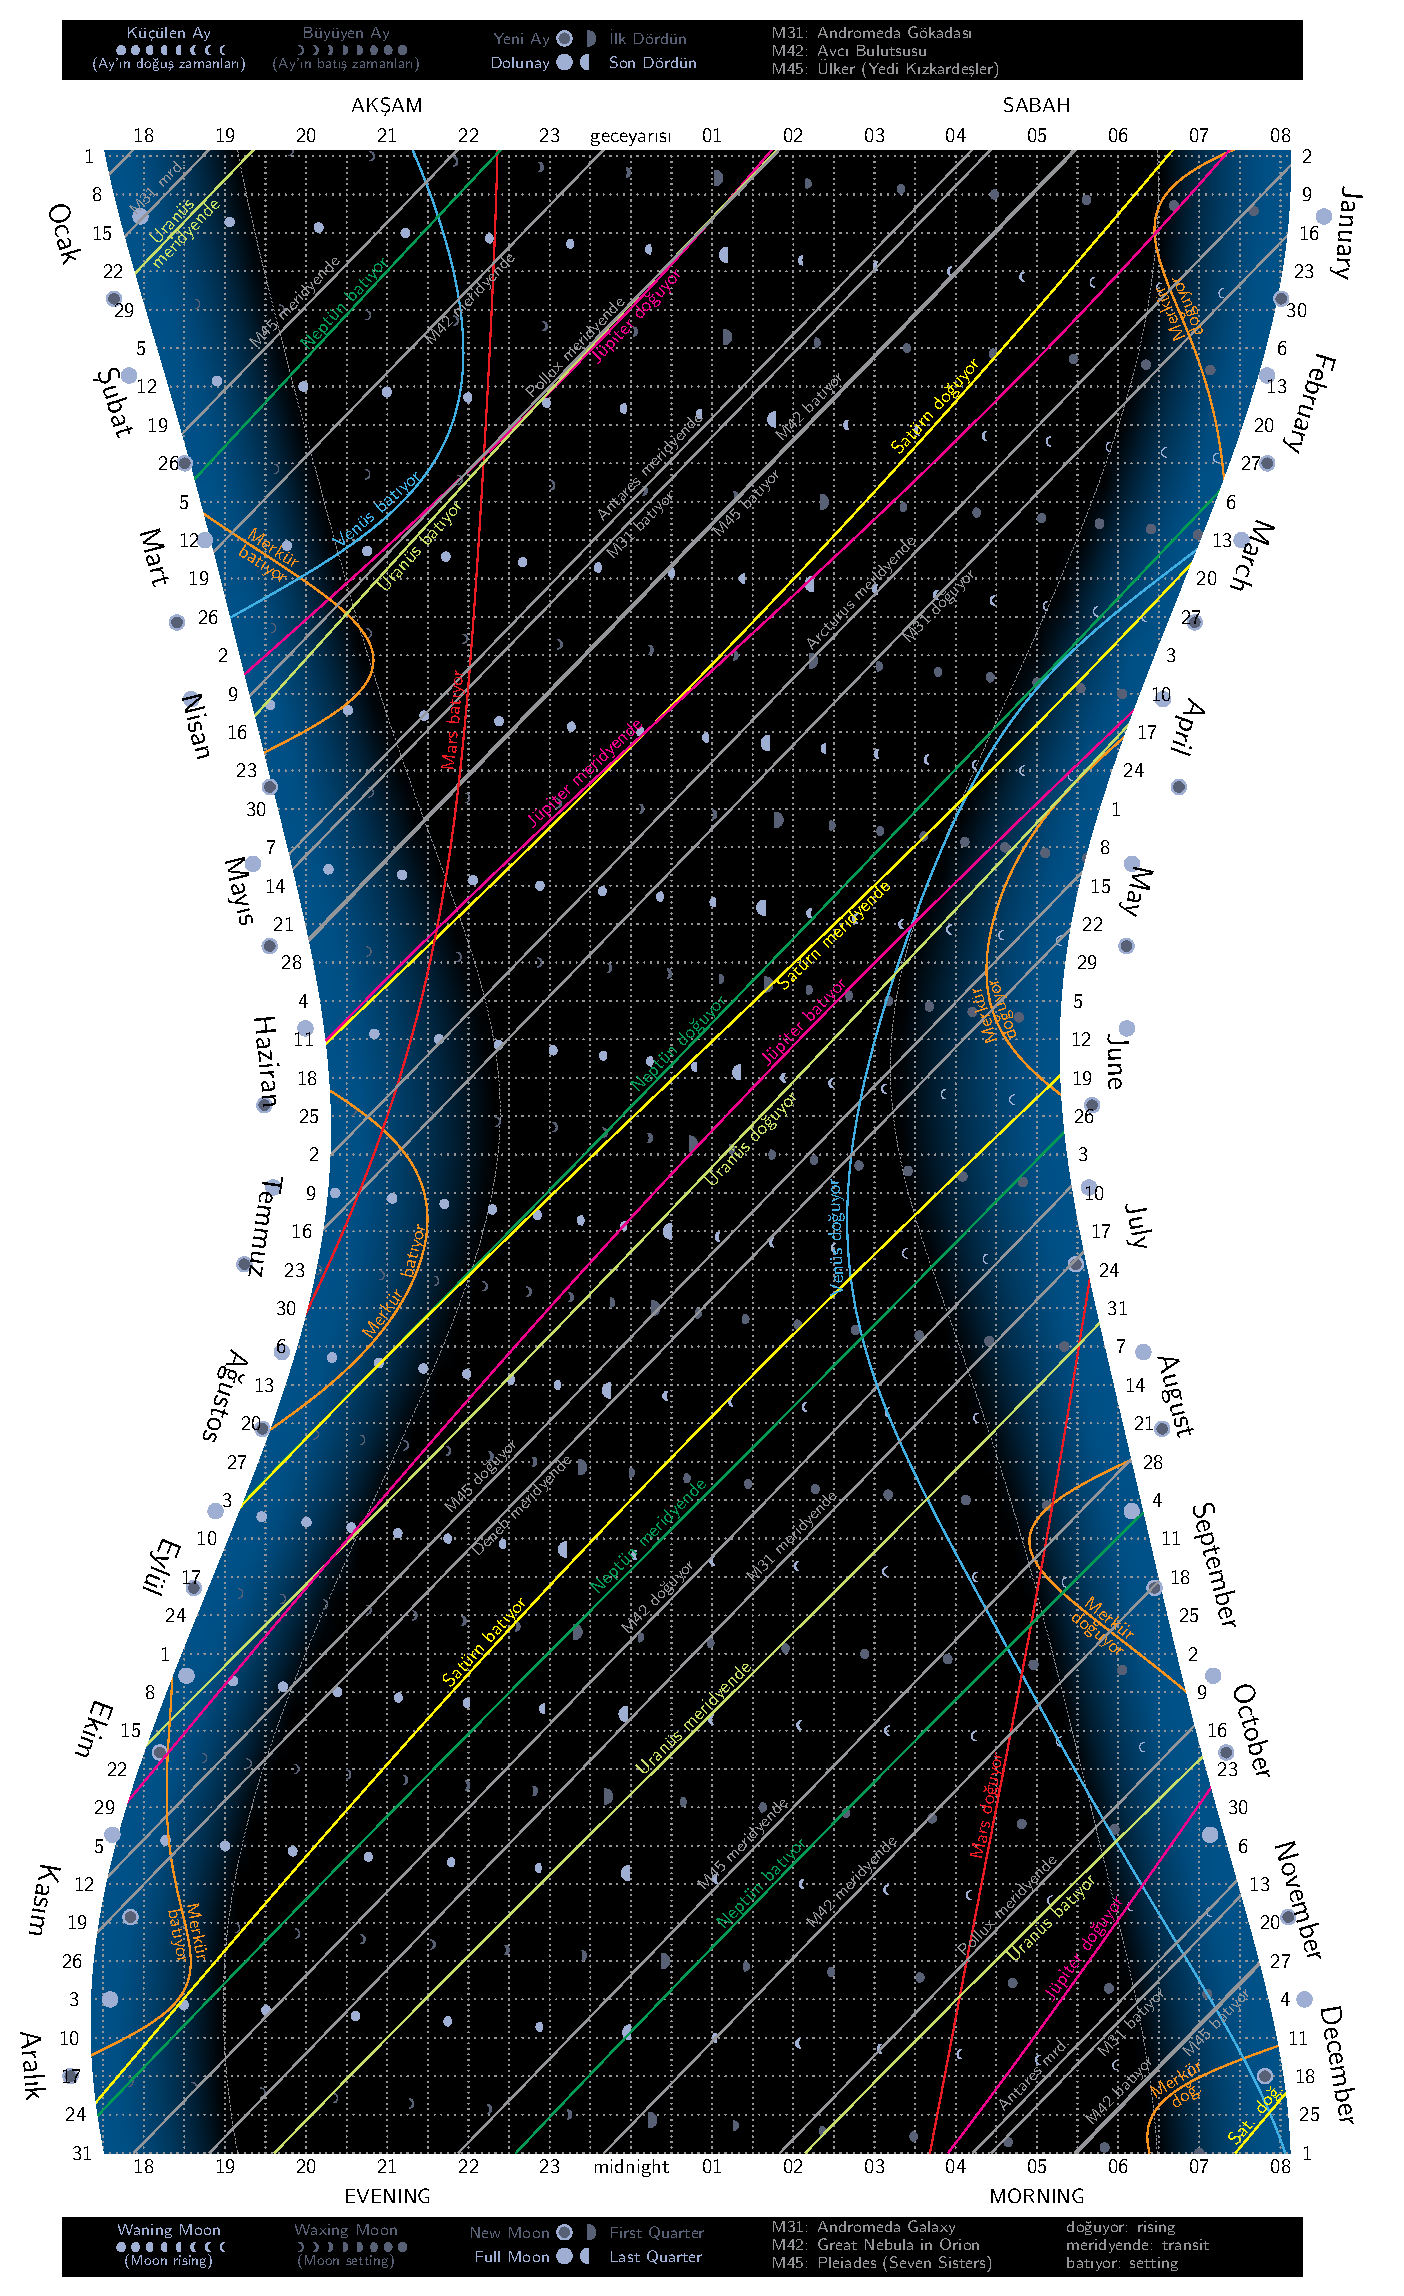
\includegraphics[clip,height=0.9\textheight]{almanac_2017_ODTU_Fizik}}

\vskip -0.9\textheight \vskip9cm
\noindent
\cutout{l}(0cm,0pt)
\shapepar{\almleftshape}{\fontsize{13pt}{13pt}\selectfont
\selectlanguage{turkish}
\hskip0.1cm\textbf{Çizelgenin Kullanımı}\\
Bu çizelge 2017 yılı için Orta Doğu Teknik Üniversitesi'nde çeşitli
gök cisimlerinin doğma, meridyenden (gökyüzünde ulaştıkları en
yüksek noktadan) geçme ve batma zamanlarını, alacakaranlığın
sonuyla başlangıcını ve Ay'ın evrelerini veriyor.  Dikey eksen
günleri, yatay eksen gece boyunca zamanı gösteriyor.  Gece içinde
yarımşar saatlik aralıklar ve yıl içinde Pazar akşamlarını
Pazartesi sabahlarına bağlayan geceler noktalı çizgilerle
belirtiliyor. Düşey olarak iki nokta arası bir güne, yatay olarak
iki nokta arası beş dakikaya karşılık geliyor.\\
Bir örnek olarak 17 Mart gecesinin olaylarına bakarsak: İlk olarak,
sol tarafta 19 Mart'a karşılık gelen noktanın üstünde yaklaşık
olarak 17 Mart'a karşılık gelen noktayı bulmak gerekiyor. Buradan
sağa doğru ilerlediğimizde 19:45 civarında Merkür, 20:10 civarında da
Venüs gezegenlerinin battığını görüyoruz. Bu bize aynı zamanda bu
gezegenlerin Güneş batarken batı ufkuna yakın olduklarını da söylüyor.
20:30 civarında alacakaranlık bitiyor (Güneş ufkun 18$^\circ$ altına
iniyor) ve yaklaşık 19:40'da Jüpiter
doğuyor. Bunu 20:45 civarında Pollux'un meridyenden geçmesi ve 21:00'de
Uranüs'ün batması izliyor. Bunun ardından Mars'ın batışı, Antares'in meridyenden
geçişi, M31'in batması ve Ay'ın sondördünden biraz daha büyük olarak
23:35 dolaylarında doğması geliyor. Bu sembol aynı zamanda bir sonraki
gece Ay'ın daha küçük olacağını söylüyor.
altında kaldığı anlara karşılık geliyor.\\
Çizelgede verilen doğma ve batma zamanları, ufuk çizgisinin önünde bir engel
olmadığını varsayıyor. Eğer böyle bir engel varsa, her bir
açı derecesi yükseklik için doğma zamanı 4 dakika geç, batma zamanı da
aynı miktarda erken olacak. Benzer biçimde, yüksek bir noktadan gözlem
yapıldığı için ufuk çizgisi olması gerekenin altında ise, doğma ve batma
zamanlarının düzeltilmesi gerekecek.\\
~}
\vskip -6.7cm
\cutout{r}(2em,6cm)
\shapepar{\almrightshape}{\fontsize{13pt}{13pt}\selectfont
\selectlanguage{english}
\hskip 0.6cm\textbf{Using the Chart}\\
This chart gives the rise, transit (reaching the highest point in
the sky) and setting time for various stellar objects, the end and the
beginning of the twilight, and the phases of the Moon for Middle East
Technical
University in the year 2017. The vertical axis denotes the days and
the horizontal axis denotes the time through the night. Every half
hour during the night and the nights of Sunday evenings and Monday
mornings are indicated by dotted lines.  In the vertical lines, each
point corresponds to a day; and for the horizontal lines to five minutes. \\
As an example, let's look at the night of March 17$^\textrm{th}$:
First of all, we need to find the point corresponding to March 17, just
above March 19 mark. As we proceed to the right from this point,
we see that Mercury and Venus set at around 19:45 and 20:10,
respectively. This also tells us that these planets were just above
western horizon when Sun had set. Twilight ends at around 20:30 (meaning
the Sun is 18$^\circ$ below the horizon) and at about 19:40
Jupiter rises. This is followed by Pollux's transit at 20:45 and Uranus
setting at 21:00. After this Mars sets, Antares transits, M31 sets and a
waning moon (meaning the Moon will be smaller the next night)
slightly larger than a last quarter at about 23:35.\\
The rise and set times in the chart are calculated by assuming that
there is no obstacle in front of the horizon. If there is such an
obstacle, for each degree angle of its height rising time will be 4
minutes late and setting time 4 minutes early. Likewise, if the horizon
is below horizontal, an adjustment has to be made.\\ ~}
\vskip 48.5cm \footnotesize

{\hfill M. Atakan Gürkan \url{<agurkan@metu.edu.tr>}}

{\hfill \url{https://github.com/atakan/PySkyAlmanac/}}
\end{document}
